\chapter{State of the Art} % Main chapter title

\label{Chapter3} % Change X to a consecutive number; for referencing this chapter elsewhere, use \ref{ChapterX}


\section{Introduction}\label{sec:Introduction}

\todosection

\section{Software Solutions}\label{sec:SoftwareSolutions}

While there are many applications in existence that allow a user to remotely control a computer from another location, few of them offer the power required to stream high-performing applications to a remote device.
The following subsections will introduce existing attempts to solve this problem as well as drawbacks that come with each implementation.


\subsection{Remote Desktop Protocol}\label{subsec:RemoteDesktopProtocol}

Microsoft's Remote Desktop Protocol (RDP), is a protocol that defines communication between a terminal server and terminal server client for multimedia purposes \cite{rdpDocs}.
Coming pre-installed on every Windows machine since Windows XP and with clients available for Windows, Mac, and Linux, RDP is an easy to use solution for remotely accessing Windows machines graphically. 

Although it is the built-in solution for Windows machines, it isn't without it's drawbacks.
Firstly, only one graphical session is active at one time while using windows.
This means if a user is logged into the host computer and someone initiates a connection with RDP, the user using the host computer will be logged out.
While this isn't always an issue, sensitive programs that don't take well to being logged out may run into issues.
Secondly, RDP does not support relative mouse movement \cite{burgin_2013}.
This means every mouse input is sent to the host computer as an absolute position on the screen, rather than as a relative distance from it's previous location.
Again, while this isn't always an issue, any application that moves the mouse for the user, such as controlling 3D applications or anything dealing with virtual cameras such as animation or game development, cannot be controlled properly.


\subsection{Virtual Network Computing}\label{subsec:VirtualNetworkComputing}

Virtual Network Computing (VNC), is a platform-independent system originally developed by Olivetti \& Oracle Research Labs and later bought and shelved by AT\&T \cite{vncFlavors}.
While the original implementation is no longer used in a wide capacity, the protocol it was developed on has been expanded and improved to become one of the most flexible yet simple ways to control a computer remotely.
VNC can run on any modern operating system, and even a web browser can serve as a VNC client.



\subsection{Chrome Remote Desktop}\label{subsec:ChromeRemoteDesktop}

\todosection


\subsection{Secure Shell Protocol}\label{subsec:SecureShellProtocol}

\todosection


\subsection{Web Clients}\label{subsec:WebClients}

\todo{https://ets.engineering.asu.edu/fse-cloud-classroom/}
\todosection


\section{Hardware Solutions}\label{sec:HardwareSolutions}

While Hardware solutions are not as popular or widespread as software solutions, there has been some innovation in the field that is worth considering.
Hardware solutions usually focus on building a device that has just enough power to connect and stream data to a remote computer in order to leverage its power for the user to use.


\subsection{Thin Clients}\label{subsec:ThinClients}

As discussed in Section \ref{sec:ThinClients}, Thin Clients are a device commonly seen in the corporate world to allow employees to access data centers and computing clusters from their desks.
Due to their low cost and ease of deployment, they are often the device of choice to enable employees to access the full power of the business' computing infrastructure without needed to purchase a powerful device for each employee.
However, since a typical thin client is a headless device, meaning it doesn't come with a monitor, keyboard, mouse, or other peripherals, they are often less portable as one might thing.
A thin client is usually set up once, and then left in that place for as long as a desktop would stay.
Especially with laptop sales on the rise, thin clients do not have the benefit of being more portable than the alternatives.

\subsection{Nvidia Shield and GameStream}\label{subsec:NvidiaShieldAndGameStream}

\begin{wrapfigure}{r}{0.375\textwidth}
  \centering
  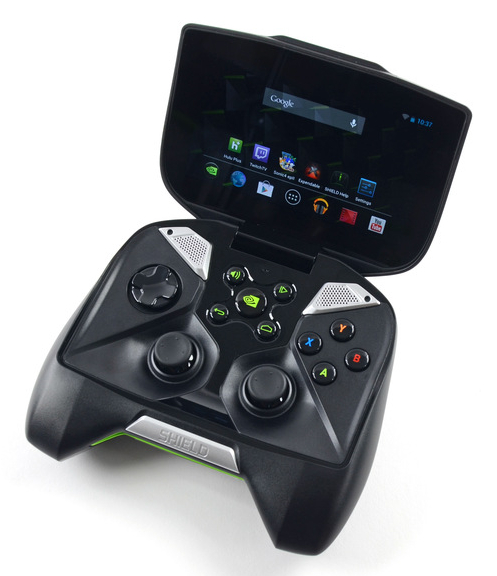
\includegraphics[width=0.3\textwidth]{Figures/nvidia-shield-open-ifixit}
  \caption[Nvidia Shield]{An open Nvidia Shield displaying the home page \cite{ImageNvidiaShield}.}
  \label{fig:nvidiashield}
\end{wrapfigure}

The Nvidia Shield game console was Nvidia's first foray into the realm of remote streaming.
Though it was focused on gaming and media streaming, it was one of the first attempts at using a portable device to stream intensive applications such as games from a host computer \cite{brown_2013}.
At the steep price point of \$349, it definitely was enthusiast hardware for a device that focused on mobile and desktop gaming over running console games or demanding titles locally.
But while the the physical device was praised for performance, battery life, and the experience of streaming games to the console, it didn't perform too well in terms of sales.
It was still widely regarded as a technological breakthrough though, and Nvidia continued to develop the technology into a new device called the Nvidia Shield TV \cite{daniel_2017}.
Focused on bringing the power of a gaming desktop to a TV, the Nvidia Shield TV dropped the idea of portability in favor of filling a different market focused on comfort.
While this is no longer a valid device for the purposes of this paper, the developments of the proprietary GameStream technology that powered the Shield and the Shield TV proved to be even more exciting than the physical devices themselves.
\todo{Does the picture look ok?}

Though the GameStream technology that powers the Nvidia Shield devices is closed source and only officially compatible with the products Nvidia releases, its enticing power and potential drew a community to reverse engineer the protocol.
In 2013, a group of students at Case Western Reserve University developed Moonlight, an open source implementation of the GameStream protocol \cite{moonlight}.
This open source implementation allows the development of GameStream compatible clients that can run on other devices, from other computers to embedded ARM devices.
This stands as a good starting place to develop the solution described in this paper.

\section{Research Questions}\label{sec:ResearchQuestions}
\todoadvisor{What are the specific questions we're trying to answer}
\todosection